%
% style = tac style
% pages = 16 
% diagram macros = tikz
% implementation of TeX = Mac Tex
%

%%%%%%%%%%%
%
%	spans of cospans
%	version.tac submission
%
%%%%%%%%%%%

%%%%%%%%%%%
%
%  preamble            
%
%%%%%%%%%%%

\documentclass{tac}

%%%%%%%%%%%
% load packages
%%%%%%%%%%%

\usepackage{amssymb, stmaryrd, etoolbox}
\usepackage{comment}
\usepackage{mathtools}
\usepackage{graphicx,caption,subcaption}

\usepackage[inline]{enumitem}
\setlist{itemsep=0em, topsep=0em, parsep=0em}
\setlist[enumerate]{label=(\alph*)}

\usepackage{tikz}
\usetikzlibrary{matrix,arrows,external}

\usepackage[colorlinks=true]{hyperref}
\hypersetup{allcolors=[rgb]{0.1,0.1,0.4}}

%%%%%%%%%%%
% tac macros
%%%%%%%%%%%

\author{Daniel Cicala}
\address{Department of Mathematics, 
	University of California, Riverside \\
	USA, 92521\\
}
\thanks{The author would like to thank John Baez 
	for many helpful discussions as well as 
	Blake Pollard and Jason Erbele for contributing 
	the Boolean algebra counterexample.}
\title {Spans of cospans}
\copyrightyear{2017}
\keywords{spans, cospans, bicategory, 
	graph rewriting, adhesive category, network theory}
\amsclass{18D05,68Q42,90B10}
\eaddress{cicala@math.ucr.edu}

%%%%%%%%%%%
% author macros
%%%%%%%%%%%

\newcommand{\cat}[1]{\mathbf{#1}}
\renewcommand{\t}[1]{\textup{#1}}
\newcommand{\from}{\colon}
\renewcommand{\span}{\xrightarrow{\mathit{sp}}}
\newcommand{\cospan}{\xrightarrow{\mathit{csp}}}
\newcommand{\csC}{\widetilde{\mathbf{C}}}

%%%%%%%%%%%
%
% begin document
%                         
%%%%%%%%%%%

\begin{document}

%%%%%%%%%%%
% 	abstract & title
%%%%%%%%%%%

\maketitle

\begin{abstract}
	We study spans of cospans in a category $ \mathbf{C} $ 
	and explain how to horizontally and vertically compose these.  
	When $ \mathbf{C} $ is a topos and the legs of the spans are monic, 
	these two forms of composition satisfy the interchange law.  
	In this case there is a bicategory of objects, cospans, and 
	`monic-legged' spans of cospans in $ \mathbf{C} $.  
	One motivation for this construction is an application to graph rewriting.
\end{abstract}

%%%%%%%%%%%
%	section:
%	introduction
%%%%%%%%%%%

\section{Introduction} 

There is currently interest in studying complex networks
through the simpler networks of which they are comprised. 
This point of view is known as \textit{compositionality}. 
Various flavors of graphs (directed, weighted, colored, etc.)
play an important role in this program because 
they are particularly well suited to model networks
\cite{Baez_CompFrameMarkovProcess,
	Baez_CompFrameLinearNetworks,
	RoseSabadinWalters_SepAlgNCospansGraphs,
	RoseSabadinWalters_CalcColimsComp}. 
By adding a bit of structure to graphs, we can decide 
how to glue graphs together to make larger graphs.  

The structure that we want to consider 
is given by choosing two subsets of nodes, 
named \textit{inputs} and \textit{outputs}. 
When the inputs of one graph equal 
the outputs of another, 
we can glue the graphs together. 
One method for adding this structure 
is to use a cospan of graphs 
	$I \to G \leftarrow O$ 
where $I$ and $O$ are discrete. 
Then gluing graphs together becomes 
a matter of composing cospans, 
which B\'{e}nabou 
	\cite{Benabou_Bicats} 
described using pushouts in the context 
of a bicategory whose morphisms are cospans 
and $2$-morphisms are maps of cospans. 
Rebro 
	\cite{Rebro_Span2} 
extended this idea to give a bicategory 
whose $2$-morphisms are cospans of cospans. 
See the figure below to see what this means.    

\begin{figure}
	\centering	
	\begin{minipage}[b]{0.3\textwidth}
	\[
		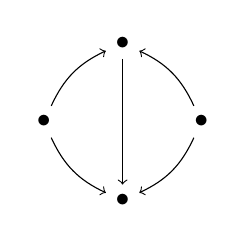
\begin{tikzpicture}
		\node (a) at (0,1) {$\bullet$};
		\node (b) at (1,0) {$\bullet$};
		\node (c) at (0,-1) {$\bullet$};
		\node (d) at (-1,0) {$\bullet$};
		%
		\path [<-] (a) edge[bend left=20] (b);
		\path [->] (b) edge[bend left=20] (c);
		\path [<-] (c) edge[bend left=20] (d);
		\path [->] (d) edge[bend left=20] (a);
		\path [->] (a) edge[] (c);
		\end{tikzpicture}
	\]
	\subcaption{Map of cospans}
	\label{fig.MapOfCospans}
	\end{minipage}
	\begin{minipage}[b]{0.3\textwidth}
	\[
		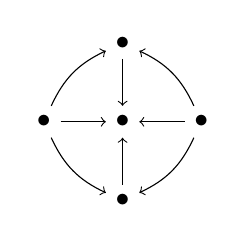
\begin{tikzpicture}
		\node (a) at (0,1) {$\bullet$};
		\node (b) at (1,0) {$\bullet$};
		\node (c) at (0,-1) {$\bullet$};
		\node (d) at (-1,0) {$\bullet$};
		\node (e) at (0,0) {$\bullet$};
		%
		\draw [<-] (a) edge[bend left=20] (b);
		\draw [->] (b) edge[bend left=20] (c);
		\draw [<-] (c) edge[bend left=20] (d);
		\draw [->] (d) edge[bend left=20] (a);
		\draw [->] (a) edge (e);
		\draw [->] (b) edge (e);
		\draw [->] (c) edge (e);
		\draw [->] (d) edge (e);
		\end{tikzpicture}
	\]
	\subcaption{Cospan of cospans}
	\label{fig.CospanOfCospans}
	\end{minipage}
	\begin{minipage}[b]{0.3\textwidth}
	\[
		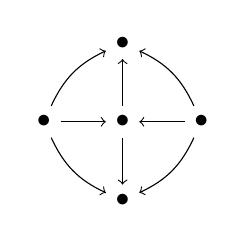
\begin{tikzpicture}
		\node (a) at (0,1) {$\bullet$};
		\node (b) at (1,0) {$\bullet$};
		\node (c) at (0,-1) {$\bullet$};
		\node (d) at (-1,0) {$\bullet$};
		\node (e) at (0,0) {$\bullet$};
		%
		\draw [<-] (a) edge[bend left=20] (b);
		\draw [->] (b) edge[bend left=20] (c);
		\draw [<-] (c) edge[bend left=20] (d);
		\draw [->] (d) edge[bend left=20] (a);
		\draw [<-] (a) edge (e);
		\draw [->] (b) edge (e);
		\draw [<-] (c) edge (e);
		\draw [->] (d) edge (e);
		\end{tikzpicture}
	\]
	\subcaption{Span of cospans}
	\label{fig.SpanOfCospans}
\end{minipage}
\caption{Various morphisms of cospans}
\end{figure}

The goal of this paper is to explore 
another tool to study networks: spans of cospans 
(see Figure \ref{fig.SpanOfCospans}). 
Grandis and Par\'{e} studied these 
in the context of intercategories 
and showed that lax interchange holds.  
We build a bicategory from certain spans of cospans.  
Both B\'{e}nabou and Rebro only required 
sufficient colimits to compose maps of cospans 
and cospans of cospans, respectively. 
For us, we require sufficient limits and colimits 
while also ensuring they play well together. 
For this reason, we start with a topos $\cat{C}$, 
then let our $0$-cells be the objects of $\cat{C}$, 
$1$-cells the cospans in $\cat{C}$, and 
$2$-cells isomorphism classes of spans 
(with monic legs) of cospans. 
Our main theorem is that this construction, 
named $\cat{MonSp(Csp(C))}$, 
really gives a bicategory. 

The specific motivation for this particular construction 
is to create a framework to house 
the rewriting of graphs (with inputs and outputs).  
Applying our construction to the topos $\cat{Graph}$ 
of presheaves on
\[
	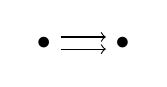
\begin{tikzpicture}
		\node (a) at (0,0) {$\bullet$};
		\node (b) at (1,0) {$\bullet$};
		\draw [->] (a.20) to (b.160);
		\draw [->] (a.-20) to (b.-160);
	\end{tikzpicture}
\]
we consider $\cat{ Rewrite }$, the full sub-bicategory 
of $\cat{ MonSp ( Csp ( Graph ) ) } $ whose objects are 
the discrete graphs. The $2$-cells of $ \cat{ Rewrite } $ 
represent all possible ways to rewrite one graph 
into another that respect the inputs and outputs. 
In this paper, graph rewrites are performed 
using the double pushout method. 
This is explained in Section \ref{sec.Rewriting}, 
though more detailed accounts exist in the literature 
	\cite{Ehrig_GraphGramAlgAp,
		LackSoboc_AdhesiveCategories}. 
Here is an example of what a $2$-cell in 
$\cat{ Rewrite }$ looks like:
\[
	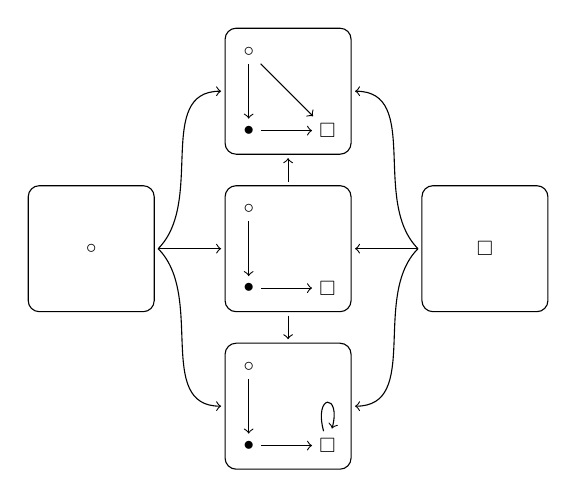
\begin{tikzpicture}
	\draw[rounded corners] (1.7,-0.3) rectangle (3.3,1.3);
	\draw[rounded corners] (1.7,1.7) rectangle (3.3,3.3);
	\draw[rounded corners] (1.7,3.7) rectangle (3.3,5.3);
	\draw[rounded corners] (-0.8,1.7) rectangle (0.8,3.3);
	\draw[rounded corners] (4.2,1.7) rectangle (5.8,3.3);
	%
	\node[scale=0.75] (ai) at (0,2.5) {$\circ$};
	\node[scale=0.75] (co) at (5,2.5) {$\square$};
	\node[scale=0.75] (a1) at (2,5) {$\circ$};
	\node[scale=0.75] (b1) at (2,4) {$\bullet$};
	\node[scale=0.75] (c1) at (3,4) {$\square$};
	\node[scale=0.75] (a2) at (2,3) {$\circ$};
	\node[scale=0.75] (b2) at (2,2) {$\bullet$};
	\node[scale=0.75] (c2) at (3,2) {$\square$};
	\node[scale=0.75] (a3) at (2,1) {$\circ$};
	\node[scale=0.75] (b3) at (2,0) {$\bullet$};
	\node[scale=0.75] (c3) at (3,0) {$\square$};
	%
	\draw [->] (a1) edge (b1);
	\draw [->] (b1) edge (c1);
	\draw [->] (a2) edge (b2);
	\draw [->] (b2) edge (c2);
	\draw [->] (a3) edge (b3);
	\draw [->] (b3) edge (c3);
	\draw [->] (a1) edge (c1);
	\draw [->] (c3) edge [loop above] (c3);
	%
	\path [->] (0.85,2.5) edge[out=0,in=180] (1.65,2.5);
	\path [->] (0.85,2.5) edge[out=45,in=180] (1.65,4.5);
	\path [->] (0.85,2.5) edge[out=-45,in=180] (1.65,0.5);
	\path [->] (4.15,2.5) edge[out=180,in=0] (3.35,2.5);
	\path [->] (4.15,2.5) edge[out=135,in=0] (3.35,4.5);
	\path [->] (4.15,2.5) edge[out=225,in=0] (3.35,0.5);
	\draw [->] (2.5,3.35) -- (2.5,3.65);
	\draw [->] (2.5,1.65) -- (2.5,1.35);
	\end{tikzpicture}
\]
Inputs are depicted with `$ \circ $', 
outputs with `$ \square $', and 
nodes depicted with `$ \bullet $' are neither. 
The picture above illustrates the rewriting 
of the top graph to the bottom graph by 
deleting an edge and adding a loop. 

The structure of this paper is as follows. 
We begin Section \ref{sec.SpansOfCospans} by 
defining spans of cospans and two ways to compose them.
When working in a topos and assuming that
the legs of the spans of cospans are monic, 
we show that the compositions satisfy an interchange law.  
This section ends with a construction of a bicategory 
whose $2$-cells are spans of cospans. 
Strictly speaking, there is no need for the full strength 
of a topos, so in Section \ref{sec.Disc on Assump}, 
we discuss how we can weaken our assumptions 
so that interchange still holds.  
Then in Section \ref{sec.Rewriting} we give a 
brief introduction to graph rewriting and 
present our motivating example: 
$\cat{ Rewrite }$, a bicategory that contains 
all possible ways to rewrite graphs.

%%%%%%%%%%%
%	section:
%	spans of cospans
%%%%%%%%%%%

\section{Spans of cospans} 
\label{sec.SpansOfCospans}

We begin by introducing spans of cospans.  
Given that our motivation is to have these be 
$2$-cells in some bicategory, 
we also show how to compose them.  
In fact, there are two ways to do so and 
these correspond to horizontal and vertical composition. 
Of course, we would like for these compositions to 
play nicely together and so we finish this section by 
showing that an interchange law holds 
under certain assumptions. 

Before we begin, a few remarks on convention are in order.
First, throughout this paper, 
tailed arrows ``$\rightarrowtail$" refer to monics, and 
two headed arrows ``$\twoheadrightarrow$" to 
quotient maps. Also, hooked arrows ``$\hookrightarrow$'' 
are canonical inclusions, which are labeled $\iota_x$ 
when its codomain is $x$. To declutter the diagrams, 
we name only those arrows that are explicitly referenced. 
Spans 
	$ A \leftarrow B \to C $
are denoted by 
	$ B \from A \span C $ 
and cospans 
	$ X \to Y \leftarrow Z $ 
by 
	$ Y \from X \cospan Z $. 
This notation is vague, but context should dispense 
with any confusion. Note that, when first defining 
spans of cospans below, the object names might seem 
to be oddly chosen. The intention is to develop a consistency
that carries into the proof of the interchange law, 
at which point, the naming should seem more methodical.

%%%%%%%%%%%%
%	subsection:
%	spans of cospans 
%	(their compositions)
%%%%%%%%%%%

\subsection{Spans of cospans and their compositions}
\label{sec:SpCspCompose}

Suppose that we are working in a category $\cat{ C }$. 
Given a parallel pair of cospans 
	$ L $, $ S \from X \cospan Y $, 
a \emph{span of cospans} is a span 
	$ S ' \from L \span S $ 
such that
\[
	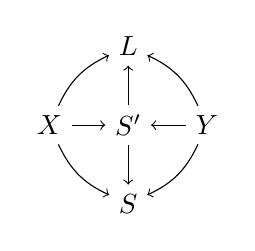
\begin{tikzpicture}
	\node (a) at (0,1) {$L$};
	\node (b) at (1,0) {$Y$};
	\node (c) at (0,-1) {$S$};
	\node (d) at (-1,0) {$X$};
	\node (e) at (0,0) {$S'$};
	%
	\draw [<-] (a) edge[bend left=20] (b);
	\draw [->] (b) edge[bend left=20] (c);
	\draw [<-] (c) edge[bend left=20] (d);
	\draw [->] (d) edge[bend left=20] (a);
	\draw [<-] (a) edge (e);
	\draw [->] (b) edge (e);
	\draw [<-] (c) edge (e);
	\draw [->] (d) edge (e);
	\end{tikzpicture}
\]
commutes. Given spans of cospans 
	$ S '_1 , S '_2 \from L \span S $, 
then a morphism of spans of cospans 
is a $\cat{C}$-morphism 
	$ S '_1 \to S '_2 $ 
such that the diagram
	\begin{equation} \label{diag.2-cell iso}
		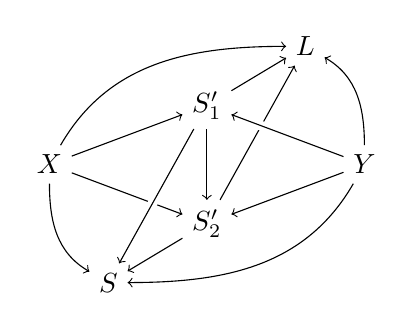
\begin{tikzpicture}
		\node (X) at (-2,0) {$X$};
		\node (L) at (1.25,1.5) {$L$};
		\node (Y) at (2,0) {$Y$};
		\node (S) at (-1.25,-1.5) {$S$};
		\node (S'1) at (0,0.75) {$S'_1$};
		\node (S'2) at (0,-0.75) {$S'_2$};
		%
		\draw [->] (X) edge[in=180,out=60] (L);
		\draw [->] (X) edge[] (S'1);
		\draw [->] (X) edge[] (S'2);
		\draw [->] (X) edge[out=-90,in=150] (S);
		\draw [->] (Y) edge[out=90,in=-30] (L);
		\draw [->] (Y) edge[] (S'2);
		\draw [->] (Y) edge[out=-120,in=0] (S);
		\draw [->] (S'1) edge[] (L);
		\draw [->] (S'1) edge[white,line width=3.5pt] (S);
		\draw [->] (S'1) edge[] (S);
		\draw [->] (S'1) edge[] (S'2);
		\draw [->] (S'2) edge[] (L);
		\draw [->] (S'2) edge[] (S);
		\draw [->] (Y) edge[white,line width=3.5pt] (S'1);
		\draw [->] (Y) edge[] (S'1);
		\end{tikzpicture}
	\end{equation}
commutes. This is an isomorphism of 
spans of cospans exactly when 
the  $\cat{ C }$-morphism is.
 
There are two different ways to turn 
compatible pairs of spans of cospans into 
a single span of cospans.  
Actually, we are foreshadowing that 
spans of cospans are $2$-cells in a bicategory. 
Therefore, we immediately name these assignments 
for what they are: vertical and horizontal composition. 
For the compositions to be defined, $\cat{ C }$ 
should have enough limits and colimits. 
Also, for the present moment, compositions are 
only be defined up to isomorphism. 
We also hold off on looking for the typical properties
composition should satisfy until we introduce 
the bicategorical structure. 

Take a pair of spans of cospans 
	$ S ' \from L \span S $ 
and 
	$ S '' \from S \span L ' $. 
Define \textit{vertical composition} $ \circ_v $ by 
	\begin{equation} \label{eq.VertComp}
			S'' \circ_v S' \coloneqq S' \times_S S'' \from L \span L'.
	\end{equation}
Diagrammatically, this is
\[
	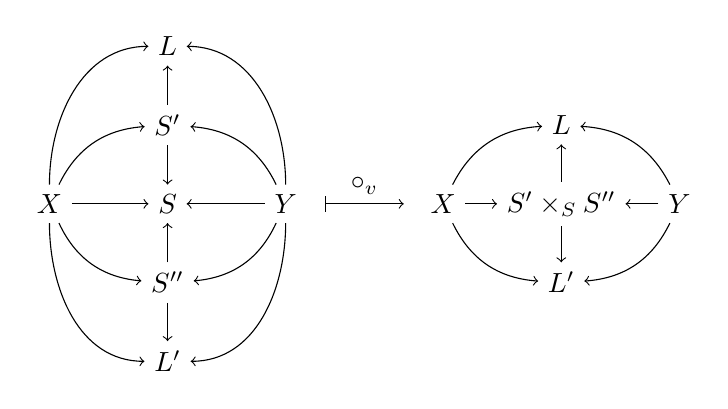
\begin{tikzpicture}
	\node (X) at (-4,0) {$X$};
	\node (Y) at (-1,0) {$Y$};
	\node (L) at (-2.5,2) {$L$};
	\node (S') at (-2.5,1) {$S'$};
	\node (S) at (-2.5,0) {$S$};
	\node (S'') at (-2.5,-1) {$S''$};
	\node (L') at (-2.5,-2) {$L'$};
	%
	\draw [->] (X) edge[out=90,in=180] (L);
	\draw [->] (X) edge[bend left=30] (S');
	\draw [->] (X) edge (S);
	\draw [->] (X) edge[bend right=30] (S'');
	\draw [->] (X) edge[out=-90,in=180] (L');
	\draw [->] (Y) edge[out=90,in=0] (L);
	\draw [->] (Y) edge[bend right=30] (S');
	\draw [->] (Y) edge (S);
	\draw [->] (Y) edge[bend left=30] (S'');
	\draw [->] (Y) edge[out=-90,in=0] (L');
	\draw [->] (S') edge (L);
	\draw [->] (S') edge (S);
	\draw [->] (S'') edge (S);
	\draw [->] (S'') edge (L');
	%-------------------------------
	\draw [|->] (-0.5,0) -- node[above] {$\circ_v$} (0.5,0);
	%-------------------------------
	\node (X) at (1,0) {$X$};
	\node (Y) at (4,0) {$Y$};
	\node (L) at (2.5,1) {$L$};
	\node (L') at (2.5,-1) {$L'$};
	\node (Spb) at (2.5,0) {$S' \times_S S''$};
	%
	\draw [->] (X) edge[bend left=30] (L);
	\draw [->] (X) edge[] (Spb);
	\draw [->] (X) edge[bend right=30] (L');
	\draw [->] (Y) edge[bend right=30] (L);
	\draw [->] (Y) edge[] (Spb);
	\draw [->] (Y) edge[bend left=30] (L');
	\draw [->] (Spb) edge[] (L);
	\draw [->] (Spb) edge[] (L');
	\end{tikzpicture}
\]
Now, let 
	$ L , S \from X \cospan Y $ 
and 
	$ R , T \from Y \cospan Z $ 
be cospans and let 
	$ S ' \from L \span S $ 
and 
	$ T ' \from R \span T $  
be spans of cospans.  Define the assignment 
\textit{horizontal composition} $ \circ_h $ by 
	\begin{equation} \label{eq.HorComp}
		T' \circ_h S' \coloneqq 
		S' +_Y T'' \from L +_Y R \span S +_Y T,
	\end{equation} 
which corresponds to 
\[
	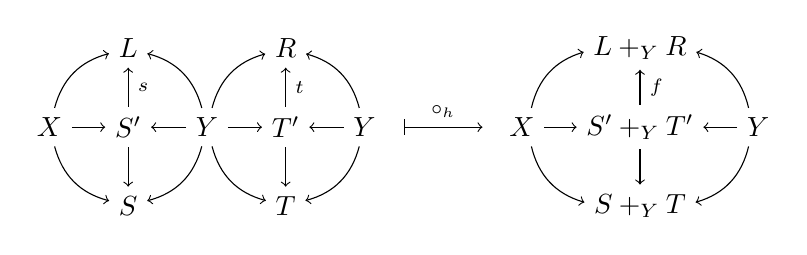
\begin{tikzpicture}
	\node (X) at (-5,0) {$X$};
	\node (Y) at (-3,0) {$Y$};
	\node (Z) at (-1,0) {$Y$};
	\node (L) at (-4,1) {$L$};
	\node (S') at (-4,0) {$S'$};
	\node (S) at (-4,-1) {$S$};
	\node (R) at (-2,1) {$R$};
	\node (T') at (-2,0) {$T'$};
	\node (T) at (-2,-1) {$T$};
	%
	\draw [->] (X) edge[bend left=30] (L);
	\draw [->] (X) edge (S');
	\draw [->] (X) edge[bend right=30] (S);
	\draw [->] (Y) edge[bend right=30] (L);
	\draw [->] (Y) edge (S');
	\draw [->] (Y) edge[bend left=30] (S);
	\draw [->] (Y) edge[bend left=30] (R);
	\draw [->] (Y) edge (T');
	\draw [->] (Y) edge[bend right=30] (T);
	\draw [->] (Z) edge[bend right=30] (R);
	\draw [->] (Z) edge (T');
	\draw [->] (Z) edge[bend left=30] (T);
	\draw [font=\scriptsize,->] (S') edge node[right] {$s$} (L);
	\draw [->] (S') edge (S);
	\draw [font=\scriptsize,->] (T') edge node[right] {$t$} (R);
	\draw [->] (T') edge (T);
	%-------------------------------
	\draw [font=\scriptsize,|->] (-0.5,0) -- node[above] {$\circ_h$} (0.5,0);
	%-------------------------------
	\node (X) at (1,0) {$X$};
	\node (Y) at (4,0) {$Y$};
	\node (L) at (2.5,1) {$L+_YR$};
	\node (L') at (2.5,-1) {$S+_YT$};
	\node (Spb) at (2.5,0) {$S'+_YT'$};
	%
	\draw [->] (X) edge[bend left=30] (L);
	\draw [->] (X) edge[] (Spb);
	\draw [->] (X) edge[bend right=30] (L');
	\draw [->] (Y) edge[bend right=30] (L);
	\draw [->] (Y) edge[] (Spb);
	\draw [->] (Y) edge[bend left=30] (L');
	\draw [font=\scriptsize,->] (Spb) edge node[right] {$f$} (L);
	\draw [->] (Spb) edge[] (L');
	\end{tikzpicture}
\]
At this point, it is natural to ask whether 
the interchange law holds between 
vertical and horizontal composition. 
It does, but not without some further assumptions. 

%%%%%%%%%%%
%	subsection:
%	spans of cospans
%	(interchange law)
%%%%%%%%%%%

\subsection{The interchange law}

Let $\cat{C}$ be a topos with 
chosen pushouts and let both 
legs of each span of cospans be monic. 
To see examples of where the interchange law fails 
without these assumptions, see Section 
	\ref{sec.Disc on Assump}.

The first thing we want to do is to show 
that the vertical and horizontal compositions 
are well-defined, up to isomorphism. 
To this end, we give a lemma that will be 
put to work several times during the course of this section.

\lemma \label{lem.helpful little lemma}
	Given a diagram
		\begin{equation} \label{diag.helpful little lemma}
			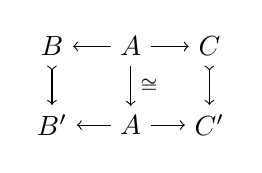
\begin{tikzpicture}
			\node (B) at (-1,1) {$B$};
			\node (A) at (0,1) {$A$};
			\node (C) at (1,1) {$C$};
			\node (B') at (-1,0) {$B'$};
			\node (A') at (0,0) {$A$};
			\node (C') at (1,0) {$C'$};
			%
			\draw [->] (A) edge (B);
			\draw [font=\scriptsize,->] (A) edge node[right] {$\cong$} (A');
			\draw [->] (A) edge (C);
			\draw [->] (A') edge (B');
			\draw [->] (A') edge (C');
			\draw [>->] (B) edge (B');
			\draw [>->] (C) edge (C');
			\end{tikzpicture}
		\end{equation}
	we get a pushout
		\begin{equation} \label{diag.helpful pushout}
			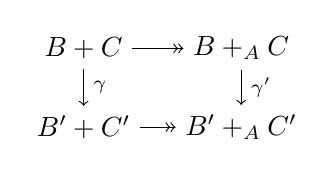
\begin{tikzpicture}
			\node (BC) at (0,1) {$B+C$};
			\node (BAC) at (2,1) {$B+_AC$};
			\node (BC') at (0,0) {$B'+C'$};
			\node (BAC') at (2,0) {$B'+_AC'$};
			%
			\draw [->>] (BC) edge (BAC);
			\draw [font=\scriptsize,->] (BC) edge node[right] {$\gamma$} (BC');
			\draw [font=\scriptsize,->] (BAC) edge node[right] {$\gamma'$} (BAC');
			\draw [->>] (BC') edge (BAC');
			\end{tikzpicture}
		\end{equation}
	such that the canonical arrows $\gamma$ and $\gamma'$ are monic.
\endlemma 
\proof
	Using its universal property, 
	we see that $\gamma$ factors through $B'+C$ as seen in diagram
	\[
		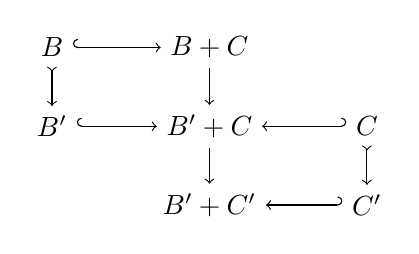
\begin{tikzpicture}
		\node (B) at (-2,1) {$B$};
		\node (B') at (-2,0) {$B'$};
		\node (BC) at (0,1) {$B+C$};
		\node (B'C) at (0,0) {$B'+C$};
		\node (B'C') at (0,-1) {$B'+C'$};
		\node (C) at (2,0) {$C$};
		\node (C') at (2,-1) {$C'$};
		%
		\draw [right hook->] (B) edge (BC);
		\draw [>->] (B) edge (B');
		\draw [right hook->] (B') edge (B'C);
		\draw [->] (BC) edge (B'C);
		\draw [->] (B'C) edge (B'C');
		\draw [left hook->] (C) edge (B'C);
		\draw [>->] (C) edge (C');
		\draw [left hook->] (C') edge (B'C');
		\end{tikzpicture}
	\]
	It is straightforward to check that the squares are both pushouts. 
	By Lemma 
		\ref{lem.adhesive properties}, 
	we get that $\gamma$ must be monic and also that 
	the monotonicity of $\gamma'$ follows from the diagram
		\eqref{diag.helpful pushout} 
	being a pushout, which we now show.
		
	One can check that the right hand square commutes 
	by using the universal property of $B+C$. 
	To see that this square is a pushout, set up a cocone $D$
		\begin{equation} \label{diag.helpful lemmma cocone}
			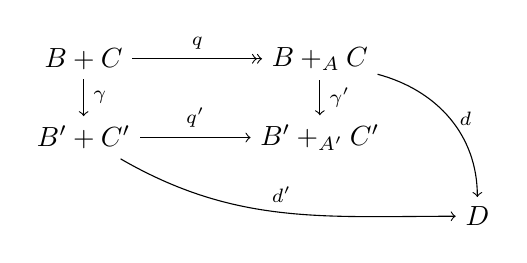
\begin{tikzpicture}[baseline=(current  bounding  box.center)]
			\node (BC) at (-1,1) {$B+C$};
			\node (BAC) at (2,1) {$B+_AC$};
			\node (BC') at (-1,0) {$B'+C'$};
			\node (BAC') at (2,0) {$B'+_{A'}C'$};
			\node (D) at (4,-1) {$D$};
			%
			\draw [font=\scriptsize,->>] (BC) edge node[above] {$q$} (BAC);
			\draw [font=\scriptsize,->] (BC) edge node[right] {$\gamma$} (BC');
			\draw [font=\scriptsize,->] (BAC) edge node[right] {$\gamma'$} (BAC');
			\draw [font=\scriptsize,->] (BAC) edge [out=-15,in=90] node[right] {$d$} (D);
			\draw [font=\scriptsize,->.] (BC') edge node[above] {$q'$} (BAC');
			\draw [font=\scriptsize,->] (BC') edge[out=-30,in=180] node[above] {$d'$} (D);
			\end{tikzpicture}
		\end{equation}
	Then $ d' \iota_{ B' }$, $ d' \iota_{ C' }$, and $ D $ form 
	a cocone under the span 
		$ B' \leftarrow A' \to C' $ 
	on the bottom face of diagram 
		\eqref{diag.helpful little lemma}. 
	This induces the canonical map 
		$ \gamma'' \from B'+_A C' \to D $.  
	It follows that 
		$ d' \iota_{ B' } = \gamma '' q' \iota_{ B' } $ 
	and 
		$ d' \iota_{ C' } = \gamma '' q' \iota_{ C' } $. 
	Therefore, $ d ' = \gamma'' q' $ by the universal property of coproducts.
		
	Furthermore, $ d q \iota_B $, $ d q \iota_C $, and $ D $ form 
	a cocone under the span 
		$ B \leftarrow A \to C $ 
	on the top face of diagram 
		\eqref{diag.helpful little lemma}. 
	Then 
		$ d q \iota_B = 
			d ' \gamma \iota_B = 
			\gamma '' q' \gamma \iota_B = 
			\gamma '' \gamma' q \iota_B$ 
	and 
		$ d q \iota_C = 
			d ' \gamma \iota_C = 
			\gamma '' q ' \gamma \iota_C = 
			\gamma '' \gamma ' q \iota_C$ 
	meaning that both $d$ and 
		$ \gamma '' \gamma ' $ 
	satisfy the canonical map 
		$ B +_A C \to D$.  
	Hence $ d = \gamma '' \gamma ' $. 
		
	The universality of $ \gamma'' $ with respect to diagram 
		\eqref{diag.helpful lemmma cocone} 
	follows from the universality of $ \gamma'' $ with respect to $ B' +_A C' $.
\endproof

\lemma
	Let
		$ S' \from L \span S $
	and
		$ S'' \from S \span L' $
	be vertically composable spans of cospans,		
	both of whose span legs are monic.
	The legs of the vertical composite span of cospans
		$ S'' \circ_v S' \from L \span L' $
	are monic. Similarly, let 
		$ L , S \from X \cospan Y $ 
	and 
		$ R , T \from Y \cospan Z $ 
	be cospans and let 
		$ S ' \from L \span S $ 
	and 
		$ T ' \from R \span T $  
	be spans of cospans with monic legs.  
	Then the legs of the horizontal composite span of cospans
		$ T' \circ_h S' \from L +_Y R \span S +_Y T $
	are monic.
\endlemma
\proof
	The result for vertical composition 
	follows from the fact that pullbacks 
	respect monics. The result for horizontal 
	composition follows from applying Lemma 
		\ref{lem.helpful little lemma} to the 
	diagrams
	\[
		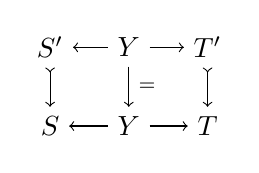
\begin{tikzpicture}
		\node (B) at (-1,1) {$S'$};
		\node (A) at (0,1) {$Y$};
		\node (C) at (1,1) {$T'$};
		\node (B') at (-1,0) {$S$};
		\node (A') at (0,0) {$Y$};
		\node (C') at (1,0) {$T$};
		%
		\draw [->] (A) edge (B);
		\draw [font=\scriptsize,->] (A) edge node[right] {$=$} (A');
		\draw [->] (A) edge (C);
		\draw [->] (A') edge (B');
		\draw [->] (A') edge (C');
		\draw [>->] (B) edge (B');
		\draw [>->] (C) edge (C');
		\end{tikzpicture}
		\quad
		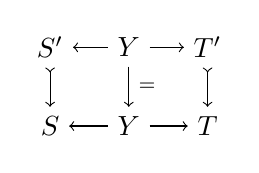
\begin{tikzpicture}
		\node (B) at (-1,1) {$S'$};
		\node (A) at (0,1) {$Y$};
		\node (C) at (1,1) {$T'$};
		\node (B') at (-1,0) {$S$};
		\node (A') at (0,0) {$Y$};
		\node (C') at (1,0) {$T$};
		%
		\draw [->] (A) edge (B);
		\draw [font=\scriptsize,->] (A) edge node[right] {$=$} (A');
		\draw [->] (A) edge (C);
		\draw [->] (A') edge (B');
		\draw [->] (A') edge (C');
		\draw [>->] (B) edge (B');
		\draw [>->] (C) edge (C');
		\end{tikzpicture}
%		\qedhere
	\]
\endproof

The interchange law requires that, given composable spans of cospans
	\begin{equation} \label{diag.2cells interchanged}
		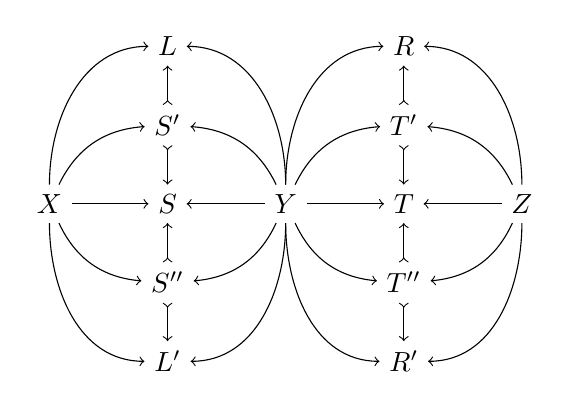
\begin{tikzpicture}
		\node (X) at (-4,0) {$X$};
		\node (Y) at (-1,0) {$Y$};
		\node (Z) at (2,0) {$Z$};
		\node (L) at (-2.5,2) {$L$};
		\node (S') at (-2.5,1) {$S'$};
		\node (S) at (-2.5,0) {$S$};
		\node (S'') at (-2.5,-1) {$S''$};
		\node (L') at (-2.5,-2) {$L'$};
		\node (R) at (0.5,2) {$R$};
		\node (T') at (0.5,1) {$T'$};
		\node (T) at (0.5,0) {$T$};
		\node (T'') at (0.5,-1) {$T''$};
		\node (R') at (0.5,-2) {$R'$};
		%
		\draw [->] (X) edge[out=90,in=180] (L);
		\draw [->] (X) edge[bend left=30] (S');
		\draw [->] (X) edge (S);
		\draw [->] (X) edge[bend right=30] (S'');
		\draw [->] (X) edge[out=-90,in=180] (L');
		\draw [->] (Y) edge[out=90,in=0] (L);
		\draw [->] (Y) edge[bend right=30] (S');
		\draw [->] (Y) edge (S);
		\draw [->] (Y) edge[bend left=30] (S'');
		\draw [->] (Y) edge[out=-90,in=0] (L');
		\draw [->] (Y) edge[out=90,in=180] (R);
		\draw [->] (Y) edge[bend left=30] (T');
		\draw [->] (Y) edge (T);
		\draw [->] (Y) edge[bend right=30] (T'');
		\draw [->] (Y) edge[out=-90,in=180] (R');
		\draw [->] (Z) edge[out=90,in=0] (R);
		\draw [->] (Z) edge[bend right=30] (T');
		\draw [->] (Z) edge (T);
		\draw [->] (Z) edge[bend left=30] (T'');
		\draw [->] (Z) edge[out=-90,in=0] (R');
		\draw [>->] (S') edge (L);
		\draw [>->] (S') edge (S);
		\draw [>->] (S'') edge (S);
		\draw [>->] (S'') edge (L');
		\draw [>->] (T') edge (R);
		\draw [>->] (T') edge (T);
		\draw [>->] (T'') edge (T);
		\draw [>->] (T'') edge (R');
		%
		\end{tikzpicture}
	\end{equation}
there is an isomorphism:
	\begin{equation} \label{eq.interchange equation}
		\left( S' \circ_\t{v} S'' \right) \circ_\t{h} 
		\left( T' \circ_\t{v} T'' \right) \cong
		\left( S' \circ_\t{h} T' \right) \circ_\t{v} 
		\left( S'' \circ_\t{h} T'' \right).
	\end{equation}
The left hand side corresponds to first applying 
vertical composition then horizontal composition. 
The right hand side swaps the order of composition. 
This isomorphism strengthens to an equality 
when isomorphism classes of spans of cospans are 
the $2$-cells of a bicategory.

It is straightforward, using 
	\eqref{eq.VertComp} 
and 
	\eqref{eq.HorComp}, 
to see that 
	\eqref{eq.interchange equation} 
reduces to finding an isomorphism
	\begin{equation} \label{eq.interchange simplified}
		( S' \times_S S'' ) +_Y ( T' \times_T T'' )
		\cong
		( S' +_Y T' ) \times_{ S +_Y T } ( S'' +_Y T'' )
	\end{equation}
of spans of cospans.

To simplify our notation, write:
	\[\begin{array}{ll}
		 A  \coloneqq ( S' \times_S S'' ) + ( T' \times_T T'' ), &
		 A_Y  \coloneqq ( S' \times_S S'' ) +_Y ( T' \times_T T'' ) , \\
		 B  \coloneqq ( S' + T' ) \times_{ S + T } ( S'' + T'' ),  &
		 B_Y  \coloneqq ( S' +_Y T' ) \times_{ S +_Y T } ( S'' +_Y T'' ).   \\
	\end{array}\]
Now, apply Lemma \ref{lem.helpful little lemma} to the diagram
\[ 
	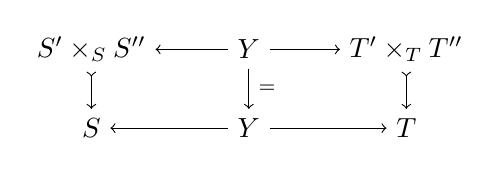
\begin{tikzpicture}
	\node (B) at (-2,1) {$S'\times_SS''$};
	\node (A) at (0,1) {$Y$};
	\node (C) at (2,1) {$T'\times_TT''$};
	\node (B') at (-2,0) {$S$};
	\node (A') at (0,0) {$Y$};
	\node (C') at (2,0) {$T$};
	%
	\draw [->] (A) edge (B);
	\draw [font=\scriptsize,->] (A) edge node[right] {$=$} (A');
	\draw [->] (A) edge (C);
	\draw [->] (A') edge (B');
	\draw [->] (A') edge (C');
	\draw [>->] (B) edge (B');
	\draw [>->] (C) edge (C');
	\end{tikzpicture}
\]
to get the pushout
\[
	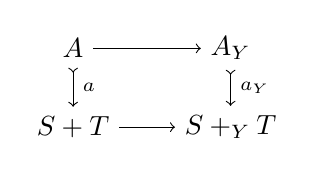
\begin{tikzpicture}
	\node (BC) at (0,1) {$A$};
	\node (BAC) at (2,1) {$A_Y$};
	\node (BC') at (0,0) {$S+T$};
	\node (BAC') at (2,0) {$S+_YT$};
	%
	\draw [->] (BC) edge (BAC);
	\draw [font=\scriptsize,>->] (BC) edge node[right] {$a$} (BC');
	\draw [font=\scriptsize,>->] (BAC) edge node[right] {$a_Y$} (BAC');
	\draw [->] (BC') edge (BAC');
	\end{tikzpicture}
\]
Similarly, we get pushouts
\[
	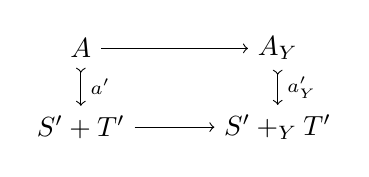
\begin{tikzpicture}[baseline=(current  bounding  box.center)]
	\node (BC) at (0,1) {$A$};
	\node (BAC) at (2.5,1) {$A_Y$};
	\node (BC') at (0,0) {$S'+T'$};
	\node (BAC') at (2.5,0) {$S'+_YT'$};
	%
	\draw [->] (BC) edge (BAC);
	\draw [font=\scriptsize,>->] (BC) edge node[right] {$a'$} (BC');
	\draw [font=\scriptsize,>->] (BAC) edge node[right] {$a'_Y$} (BAC');
	\draw [->] (BC') edge (BAC');
	\end{tikzpicture}
	\quad
	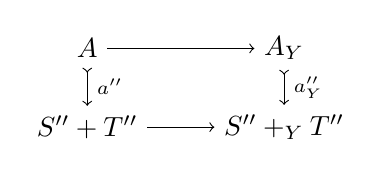
\begin{tikzpicture}
	\node (BC) at (0,1) {$A$};
	\node (BAC) at (2.5,1) {$A_Y$};
	\node (BC') at (0,0) {$S''+T''$};
	\node (BAC') at (2.5,0) {$S''+_YT''$};
	%
	\draw [->] (BC) edge (BAC);
	\draw [font=\scriptsize,>->] (BC) edge node[right] {$a''$} (BC');
	\draw [font=\scriptsize,>->] (BAC) edge node[right] {$a''_Y$} (BAC');
	\draw [->] (BC') edge (BAC');
	\end{tikzpicture}
\]
Now, $A$  forms a cone over the cospan 
	$ S + T \from S' + T' \cospan S'' + T''$ 
via the maps $ a $, $ a' $, and $ a'' $. 
And so, we get a canonical map 
	$ \theta \from A \to B $.  

\lemma \label{lem:pullback over subobject}
	Given cospans 
		$ Y $, $ W \from X \cospan Z $ 
	where the legs of $W$ factor through a monic 
		$Y \rightarrowtail W $, 
	then there is a unique isomorphism 
		$ X \times_Y Z \cong X \times_W Z $. 
\endlemma
\proof
	Via the projection maps, 
		$X \times_Y Z$ 
	forms a cone over the cospan 
		$ W \from X \cospan Z $ 
	and, also, $X \times_W Z$ forms a 
	cone over the cospan 
		$ Y \from X \cospan Z $, 
	though the latter requires the monic 
		$ Y \rightarrowtail W $ 
	to do so. Universality implies that the 
	induced maps are mutual inverses and 
	they are the only such pair.  
\endproof

\lemma \label{lem.Theta Iso}
	The map $\theta \from A \to B$ is an isomorphism.
\endlemma
\proof
	Because colimits are stable under pullback 
		\cite[Thm.~4.7.2]{MacLaneMoerdijk_SheavesGeomLogic}, 
	we get an isomorphism
	\[
		\gamma \from 
			( S'\times_{ S + T } S'' ) +
			( S'\times_{ S + T } T'' ) +
			( T'\times_{ S + T } S'' ) +
			( T'\times_{ S + T } T'' ) 
			\to B.
	\]
	But 
		$ S' \times_{ S + T } T'' $ 
	and 
		$ S'' \times_{ S + T } T' $ 
	are initial. To see this, recall that in a topos, 
	all maps to the initial object are isomorphisms. 
	Now, consider the diagram
	\[
		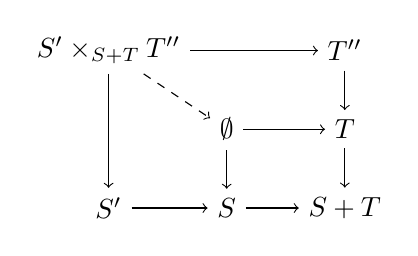
\begin{tikzpicture}
		\node (STpb) at (0,2) {$S' \times_{S+T} T''$};
		\node (T'') at (3,2) {$T''$};
		\node (0) at (1.5,1) {$\emptyset$};
		\node (T) at (3,1) {$T$};
		\node (S') at (0,0) {$S'$};
		\node (S) at (1.5,0) {$S$};
		\node (ST) at (3,0) {$S+T$};
		%
		\draw [->] (STpb) edge (S');
		\draw [->] (STpb) edge (T'');
		\draw [->] (STpb) edge[dashed] (0);
		\draw [->] (0) edge (S);
		\draw [->] (0) edge (T);
		\draw [->] (S) edge (ST);
		\draw [->] (T) edge (ST);
		\draw [->] (S') edge (S);
		\draw [->] (T'') edge (T);
		\end{tikzpicture}
	\]
	whose lower right square is a pullback because 
	coproducts are disjoint in topoi.  Similarly, 
		$ T' \times_{ S + T } S'' $ 
	is initial.  Hence we get a canonical isomorphism
		\begin{equation} \label{eq:B second iso}
			\gamma' \from 
			( S' \times_{ S + T } S'' ) + ( T' \times_{ S + T } T'' ) 
			\to B
		\end{equation}
	that factors through $\gamma$. But Lemma 
		\ref{lem:pullback over subobject} 
	gives unique isomorphisms 
		$ S' \times_{ S } S'' \cong S' \times_{ S + T } S''$ 
	and 
		$ T' \times_{ T } T'' \cong T' \times_{ S + T } T''$. 
	This produces a canonical isomorphism 
	\[
		\gamma'' \from 
			A \to ( S' \times_{ S + T } S'' ) + ( T' \times_{ S + T } T'' ).
	\]
	One can show that 
		$ \theta = \gamma' \circ \gamma'' $ 
	using universal properties.  
\endproof

Now, let us consider the following diagram:
	\begin{equation} \label{diag.the big cube}
		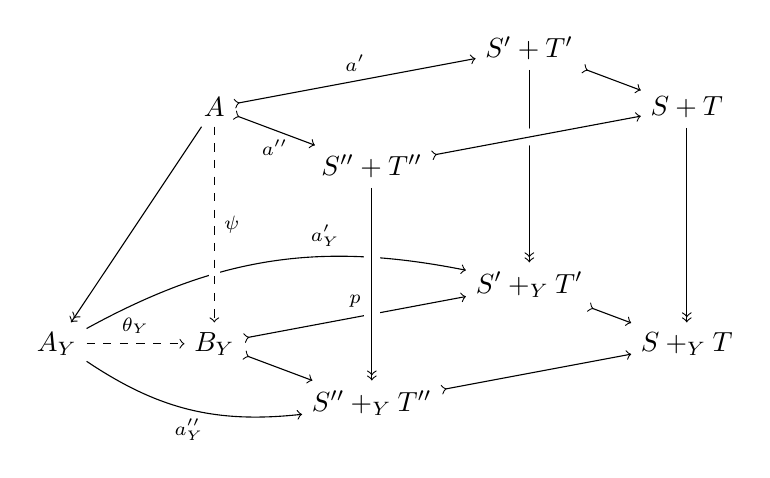
\begin{tikzpicture}
		\node (A) at (2,3) {$A$};
		\node (Ay) at (0,0) {$A_Y$};
		\node (By) at (2,0) {$B_Y$};
		\node (ST) at (8,3) {$S+T$};
		\node (ST') at (6,3.75) {$S'+T'$};
		\node (ST'') at (4,2.25) {$S''+T''$};
		\node (SYT) at (8,0) {$S+_YT$};
		\node (SYT') at (6,0.75) {$S'+_YT'$};
		\node (SYT'') at (4,-0.75) {$S''+_YT''$};
		%
		\draw [->>] (A) edge (Ay);
		\draw [font=\scriptsize,>->] (A) edge node[below] {$a''$} (ST'');
		\draw [font=\scriptsize,>->] (A) edge node[above] {$a'$} (ST');
		\draw [font=\scriptsize,->] (Ay) edge[bend left=20,pos=0.65] node[above] {$a'_Y$} (SYT');
		\draw [font=\scriptsize,->] (Ay) edge[dashed] node[above] {$\theta_Y$} (By);
		\draw [font=\scriptsize,->] (Ay) edge[bend right=20] node[below] {$a''_Y$} (SYT'');
		\draw [font=\scriptsize,>->] (By) edge node[above] {$p$} (SYT');
		\draw [>->] (By) edge (SYT'');
		\draw [->>] (ST') edge (SYT');
		\draw [>->] (ST') edge (ST);
		\draw [>->] (ST'') edge (ST);
		\draw [->>] (ST) edge (SYT);
		\draw [>->] (SYT') edge (SYT);
		\draw [>->] (SYT'') edge (SYT);
		%
		\draw [->] (A) edge[white,line width=4pt] (By);
		\draw [font=\scriptsize,->] (A) edge[dashed] node[right] {$\psi$} (By);
		\draw [->] (ST'') edge[white,line width=6pt] (ST);
		\draw [>->] (ST'') edge (ST);
		\draw [->] (ST'') edge[white,line width=6pt] (SYT'');
		\draw [->>] (ST'') edge (SYT'');
		\end{tikzpicture}
	\end{equation}
where $\theta_Y$ and $\psi$ are the canonical maps. 
Observe that $\psi$ factors through $\theta_Y$ in the above diagram.  
This follows from the universal property of pullbacks. 
We also have that the top square is a pullback from the previous lemma.

\lemma \label{lem.theta_Y iso}
	The map $ \theta_Y \from A_Y \to B_Y $ is an isomorphism.
\endlemma
\proof
	Because we are working in a topos, 
	it suffices to show that $\theta_Y$ is both monic and epic. 
	It is monic because $a'_Y$ is monic.
	
	To see that $\theta_Y$ is epic, 
	it suffices to show that $\psi$ is epic. 
	The front and rear right faces of 
		\eqref{diag.the big cube} 
	are pushouts by Lemma 
		\ref{lem.helpful little lemma}.  
	Then because the top and bottom squares of 
		\eqref{diag.the big cube} 
	are pullbacks consisting of only monomorphisms, 
	Lemma \ref{lem.vk dual} implies that the front 
	and rear left faces are pushouts.  
	However, as pushouts over monos, Lemma 
		\ref{lem.adhesive properties} 
	tells us they are pullbacks.  But in a topos, regular epis 
	are stable under pullback, and so $\psi$ is epic.  	
\endproof

It remains to show that $\theta_Y$ serves as 
an isomorphism between spans of cospans. This 
amounts to showing that
	\begin{equation} \label{diag.theta 2-cell iso}
		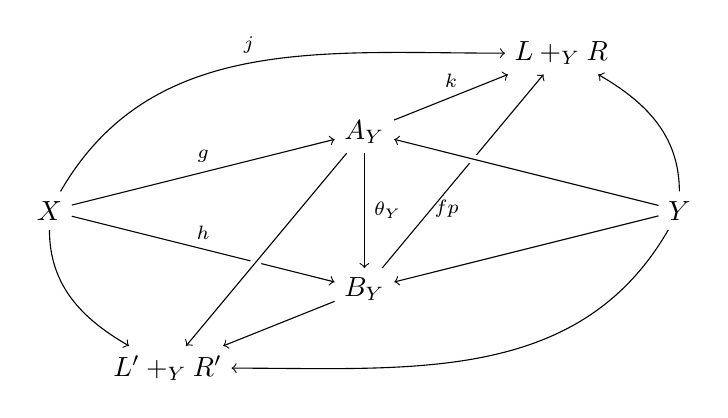
\begin{tikzpicture}
		\node (X) at (-4,0) {$X$};
		\node (LyR) at (2.5,2) {$L+_YR$};
		\node (Y) at (4,0) {$Y$};
		\node (LyR') at (-2.5,-2) {$L'+_YR'$};
		\node (Ay) at (0,1) {$A_Y$};
		\node (By) at (0,-1) {$B_Y$};
		%
		\draw [font=\scriptsize,->] (X) edge[in=180,out=60] node[above] {$j$} (LyR);
		\draw [font=\scriptsize,->] (X) edge node[above] {$g$} (Ay);
		\draw [font=\scriptsize,->] (X) edge node[above] {$h$} (By);
		\draw [->] (X) edge[out=-90,in=150] (LyR');
		\draw [->] (Y) edge[out=90,in=-30] (LyR);
		\draw [->] (Y) edge[] (By);
		\draw [->] (Y) edge[out=-120,in=0] (LyR');
		\draw [font=\scriptsize,->] (Ay) edge node[above] {$k$} (LyR);
		\draw [font=\scriptsize,->] (Ay) edge node[right] {$\theta_Y$} (By);
		\draw [font=\scriptsize,->] (By) edge[pos=0.4] node[below] {$fp$} (LyR);
		\draw [->] (By) edge[] (LyR');
		%
		\draw [->] (Y) edge[white,line width=3.5pt] (Ay);
		\draw [->] (Y) edge[] (Ay);
		\draw [->] (Ay) edge[white,line width=3.5pt] (LyR');
		\draw [->] (Ay) edge[] (LyR');
		\end{tikzpicture}
	\end{equation}
commutes. Here $g$ and $k$ are induced from 
applying vertical composition before horizontal, 
$h$ from applying horizontal composition before vertical, 
$j$ is from composing in either order, $f$ is from 
	 \eqref{eq.HorComp}, 
and $p$ is from 
	\eqref{diag.the big cube}.  
The top and bottom face commute by construction.

\lemma
	The inner triangles of diagram 
		\eqref{diag.theta 2-cell iso} 
	commute. That is, we have 
		$ k = f p  \theta_Y$ 
	and 
		$ h = \theta_Y g $.
\endlemma
\proof	
	To see that 
		$ k = f p \theta_Y $, 
	consider the diagram
	\[
		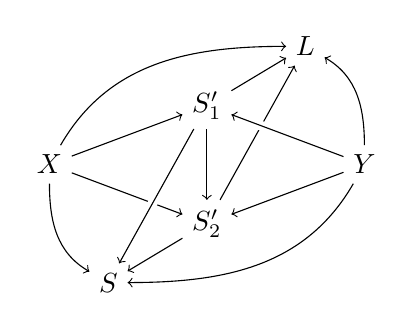
\begin{tikzpicture}
		\node (X) at (-2,0) {$X$};
		\node (L) at (1.25,1.5) {$L$};
		\node (Y) at (2,0) {$Y$};
		\node (S) at (-1.25,-1.5) {$S$};
		\node (S'1) at (0,0.75) {$S'_1$};
		\node (S'2) at (0,-0.75) {$S'_2$};
		%
		\draw [->] (X) edge[in=180,out=60] (L);
		\draw [->] (X) edge[] (S'1);
		\draw [->] (X) edge[] (S'2);
		\draw [->] (X) edge[out=-90,in=150] (S);
		\draw [->] (Y) edge[out=90,in=-30] (L);
		\draw [->] (Y) edge[] (S'2);
		\draw [->] (Y) edge[out=-120,in=0] (S);
		\draw [->] (S'1) edge[] (L);
		\draw [->] (S'1) edge[white,line width=3.5pt] (S);
		\draw [->] (S'1) edge[] (S);
		\draw [->] (S'1) edge[] (S'2);
		\draw [->] (S'2) edge[] (L);
		\draw [->] (S'2) edge[] (S);
		\draw [->] (Y) edge[white,line width=3.5pt] (S'1);
		\draw [->] (Y) edge[] (S'1);
		\end{tikzpicture}
	\]
	The bottom face is exactly the pushout diagram 
	from which $f$ was obtained.  Universality implies that 
		$ k = f a'_Y $ 
	and, as seen in 
		\eqref{diag.the big cube}, 
	$ a'_Y = p \theta_Y $. 
	
	That 
		$ h = \theta_Yg $ 
	follows from 
	\[
		f p h 
			= j
			= k g 
			= f p \theta_Y g
	\] 
	and the fact that $ f p $ is monic.
\endproof

Of course, we have only shown that 
two of the four inner triangles commute, 
but we can replicate our arguments to s
how the remaining two commute as well.  
This lemma was the last step in proving the following interchange law.

\theorem \label{thm.interchange law}
	Given diagram 
		\eqref{diag.2cells interchanged} 
	in a topos, there is a canonical isomorphism 
		$ ( S' \times_S S'' ) +_Y ( T' \times_T T'' ) 
			\cong 
			( S' +_Y T' ) \times_{ S +_Y T } ( S'' +_Y T'')$.
\endtheorem

Note that Section 
	\ref{sec.Disc on Assump}
contains a discussion on the assumptions
taken in this theorem.

%%%%%%%%%%%
%	section:
% 	spans of cospans
%	(construction)
%%%%%%%%%%%

\subsection{Constructing the bicategory}

Let $\cat{C}$ be any topos. 
We commence construction of a bicategory named 
	$ \cat{ Mon Sp ( Csp ( C ) ) } $, 
or $ \csC $ for short. 
The $0$-cells of $ \csC $ are just the $\cat{C}$-objects. 
For $0$-cells $X$ and $Y$, build a category $\csC(X,Y)$ 
whose objects are $\cat{C}$-cospans and 
morphisms are isomorphism classes of 
$\cat{C}$-spans of cospans whose legs are both monic. 
Composition in $ \csC ( X , Y )$ is the vertical composition $\circ_v$ 
introduced in 
	\eqref{eq.VertComp}. 
It is straightforward to check that associativity holds and 
that spans of cospans whose legs are identity serve as identities.

The composition functor is given by an assignment
\[
	\otimes \from 
		\csC(Y,Z) \times \csC(X,Y) 
		\to \csC(X,Z)
\]
that acts on $1$-cells by 
	$ ( T , S ) \mapsto S \otimes_Y T $ 
and on $2$-cells by horizontal composition $\circ_h$ from 
	\eqref{eq.HorComp}. 
It is straightforward to check that $\otimes$ preserves identities. 
Theorem 
	\ref{thm.interchange law} 
ensures that $\otimes$ preserves composition.

For every $0$-cell $X$, the identity functor 
	$ \cat{ 1 } \to \csC ( X , X ) $ 
picks out the $2$-cell with all identity maps on $X$. 
The associator is made of $2$-cells 
\[
	R +_X S +_Y T \from 
		( R +_X S ) +_Y T \span R +_X ( S +_Y T ) .
\] 
The right unitor is made of $2$-cells 
	$ S \from S +_Y Y \span S $. 
Likewise, the left unitor has $2$-cells 
	$ T \from T \span Y +_Y T $. 
The legs for each of the above are the obvious choices. 
The pentagon and triangle identities follow from 
the associativity, up to isomorphism, of pushouts. 

Given all of the data just laid out, 
we have the main theorem of the paper.

\theorem
	If $\cat{C}$ is a topos, then 
		$ \cat{MonSp ( Csp ( C ) ) } $ is a bicategory.
\endtheorem

%%%%%%%%%%%
%	section:
%	the assumptions
%%%%%%%%%%%

\section{A discussion on the assumptions}
\label{sec.Disc on Assump}

Can we expand the domain on which this construction works? 
Apart from ensuring sufficiently many limits and colimits, 
the primary source of roadblocks is the interchange law. 
As we discuss below, it is not absolutely necessary to work 
strictly within a topos, but we choose to do so in order to be expeditious.  
To lay out, one by one, the requirements for our interchange law to hold 
would be exhausting and leave us little energy to work through its proof. 
To do this is even less reasonable given the ubiquity of topoi.   
However, listing these requirements is interesting enough to take a look at here.  

Before digging deeper into the properties used, 
let's convince ourselves of the necessity 
for monic legs within our span of cospans.

\example
	Consider the category $\cat{Set}$ of sets and functions. 
	Relax the assumption that the legs of the 
	spans of cospans are both monic.  Indeed, suppose that 
	$ S' $, $ S'' $, and $ T' $ are two element sets and 
	$ S $, $ Y $, $ T $, and $ T'' $ are singletons.  
	The functions can be any of the limited choices we have.  
	After several routine calculations, we determine that 
		$ ( S' \times_S S'' ) +_Y ( T' \times_T T'' ) $ 
	has cardinality $5$ and 
		$ ( S' +_Y T' ) \times_{ S +_Y T } ( S'' +_Y T'' ) $
	has cardinality $6$. 
\endexample

So we see that even in the archetypal topos, 
the legs of the spans must be monic for the 
interchange law to hold. But even if they are, 
this law may fail if our category $C$ is not a topos. 
The next example illustrates this.

\example
	Consider the Boolean algebra on a two element set.  
	This is the category $0 \to 1$ with products given by 
	meet and coproducts given by join. 
	Note that this is not a topos. 
	Indeed, the only non-identity morphism is both monic and epic 
	but, as no inverse exists, it is not an isomorphism. 
	Recalling the interchange equation 
		\eqref{eq.interchange equation}, 
	suppose that we have 
		$ Y = S'' = T' = 0 $ 
	and 
		$ S = S' = T = T'' = 1 $.  
	It is straightforward to check that 
		$ ( S' \times_S S'' ) +_Y ( T' \times_T T'' ) = 0 $ 
	and 
		$ ( S' +_Y T' ) \times_{ S +_Y T } ( S'' +_Y T'' ) = 1 $. 
	That is, the interchange equation does not hold.  
	Because this Boolean algebra can be embedded into any other, 
	it follows that interchange does not hold for any Boolean algebra.
\endexample

Now that we are convinced that we actually do need to assume 
something for interchange to work, we can list our requirements.  
The obvious place to start is by asking for our category to have 
enough limits and colimits.  

In Lemma 
	\ref{lem.helpful little lemma}, 
we use that pushouts respect monics.  
This occurs in topoi. Indeed, this occurs in any
adhesive category, which we discuss further in Section 
	\ref{sec.Rewriting}.  

In Lemma 
	\ref{lem.Theta Iso}, 
we use several facts.  The first is that coproducts are disjoint, 
meaning that a pullback over coproduct inclusions is initial. 
We also use that colimits---particularly coproducts---are stable under pullback.  
The full force of a topos is not needed to satisfy this requirement.  
It suffices that our category is locally cartesian closed
	\cite[Thm.~1.4.9]{MacLaneMoerdijk_SheavesGeomLogic}.

In Lemma 
	\ref{lem.theta_Y iso}, 
we use that a monic epimorphism is an isomorphism in topoi. 
This is surely not true in general, but it is always true that a 
monic regular epimorphism is an isomorphism.  
Notice that the vertically aligned epimorphisms in Diagram 
	\eqref{diag.the big cube} 
are all regular since they are all coequalizers. For instance 
	$ S + T \twoheadrightarrow S +_Y T $ 
is a coequalizer over 
	$ Y \rightrightarrows S + T $. 
So we can merely ask for pullbacks to preserve regular epimorphisms. 
Note that this does happen in a regular category, 
which is a larger class than topoi.   

Also in Lemma 
	\ref{lem.theta_Y iso}, 
we make use of Lemmas 
	\ref{lem.adhesive properties} 
and 
	\ref{lem.vk dual}.  
This holds in any adhesive category. 

It is clear that the properties of adhesive categories 
(see Section \ref{sec.Rewriting})
play an important role in ensuring that $\csC$ is a bicategory, 
as does being locally cartesian closed and regular.  
Topoi are a well-known, large family of categories 
that are contained in the intersection of all of these classes. 

%%%%%%%%%%%
%	section:
%	rewriting
%%%%%%%%%%%

\section{An informal introduction to graph rewriting}
\label{sec.Rewriting}

For those who are not familiar with rewriting systems, 
and graph rewriting in particular, 
we provide a brief introduction. 
For a more in-depth and rigorous viewpoint, see 
	\cite{Baader_TermRewritingAllThat}, 
	\cite{Ehrig_GraphGramAlgAp}, or 
	\cite{LackSoboc_AdhesiveCategories}.

There are many methods of rewriting found throughout 
mathematics, computer science, and linguistics. 
The general idea is that we begin with a collection of rules, 
a collection of terms, and a way to apply rules to certain, compatible terms.  
When applied to a term, a rule replaces a sub-term with a new sub-term. 
A simple, informal example is found within the English language.  
Consider a set of rules 
\[
	\{ \t{(noun)} \mapsto x : x \t{ is an English noun} \}.
\]
We can apply any one of these rules to
\[
	\t{`The (noun) is far away.'}
\] 
to obtain heaps of grammatically correct, if potentially ridiculous sentences.  

The first rewriting methods were uni-dimensional, 
in that they are concerned with replacing a string of characters or letters. 
Many attempts to define multi-dimensional rewriting systems came up short 
in application and execution, but Ehrig, Pfender, and Scheider 
developed a categorical approach using graph morphisms and pushouts 
	\cite{Ehrig_GraphGramAlgAp} 
that has since been studied extensively. This approach came to be known as 
\textit{double pushout graph rewriting}. This is what we are interested in and 
consider in our bicategory $\cat{Rewrite}$ introduced below.

Here is how double pushout graph rewriting works. A \emph{production} is a span 
\[
	p \from L \leftarrowtail K \rightarrowtail R
\] 
of graphs with monic legs. Some authors call this a 
`linear production' to distinguish it from spans with potentially non-monic legs, 
but we do not adopt this convention here. Given a production $p$, 
and a graph morphism $L \to C$, called a \emph{matching map}, 
such that there exists a diagram
	\begin{equation} \label{diag:derivation}
		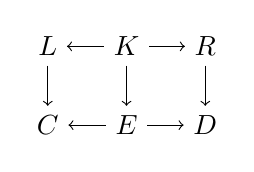
\begin{tikzpicture}
		\node (L) at (-1,1) {$L$};
		\node (K) at (0,1) {$K$};
		\node (R) at (1,1) {$R$};
		\node (C) at (-1,0) {$C$};
		\node (E) at (0,0) {$E$};
		\node (D) at (1,0) {$D$};
		%
		\draw [->] (K) edge (L);
		\draw [->] (K) edge (E);
		\draw [->] (K) edge (R);
		\draw [->] (E) edge (C);
		\draw [->] (E) edge (D);
		\draw [->] (L) edge (C);
		\draw [->] (R) edge (D);
		\end{tikzpicture}
	\end{equation}
consisting of two pushout squares, we say that that $D$ is a 
\emph{derivation} of $C$ and write 
	$ C \rightsquigarrow_E D $ 
or just 
	$ C \rightsquigarrow D $. 
The arrow `$\rightsquigarrow$' is commonly decorated
with more information: for instance, the name of the production or the matching map.  
But that is not necessary here. Observe that the objects $E$ and $D$ 
need not exist, but when they do, they are unique up to isomorphism 
	\cite[Lemma 4.5]{LackSoboc_AdhesiveCategories}. 

A \emph{grammar} 
	$ ( \mathcal{ G } , \mathcal{ P } ) $ is a set of graphs $ \mathcal{ G } $ paired with a 
set of productions $\mathcal{P}$. A \textit{derivation of the grammar} 
is a string of derivations 
\[
	G_0 \rightsquigarrow G_1 \rightsquigarrow \dotsm \rightsquigarrow G_n
\] 
from productions in $\mathcal{P}$ and with $G_0 \in \mathcal{G}$. 
We say that $G_n$ is a \emph{rewrite of $G_0$}. The \textit{language} 
	$ \mathcal{ L } ( \mathcal{ G } , \mathcal{ P } ) $ 
generated by the grammar is the collection of all graphs $G$ 
such that there is a derivation $G_0 \rightsquigarrow^\ast G$ of the grammar. 
The idea is that one would study a language. Exactly what properties are interesting 
is beyond the scope of this discussion.  Interested readers should consult the 
references mentioned at the beginning of this section.  
Instead of going deeper into the subject, we briefly zoom out.

Seeking to axiomatise graph rewriting, Lack and Sobocinski 
	\cite{LackSoboc_AdhesiveCategories} 
introduced a class of categories they call \emph{adhesive}. 
Roughly, a category is adhesive if it has pullbacks, pushouts along monomorphisms, 
and certain exactness conditions between pullbacks and pushouts hold. 
These exactness conditions, while subtle, imply all the properties one wants in double pushout rewriting.

Given that topoi are adhesive 
	\cite{LackSoboc_ToposesAdhesive},
there are many examples of adhesive categories. 
One advantage of the generalization is that adhesivity is preserved under coslicing.  For instance, the category of pointed sets not a topos, but it is adhesive because it is equivalent to the coslice category $ 1 \downarrow \cat{ Set } $.

Presently, we are interested in
using the adhesivity of topoi, 
which allows us to use Lemmas
	\ref{lem.adhesive properties}
and 
	\ref{lem.vk dual}, 
in our construction. 
While originally proved for adhesive categories,
we restrict our assumptions to topoi as this suits our needs.                                 

\lemma[{\cite[Lemmas 4.2-3]{LackSoboc_AdhesiveCategories}}] 
\label{lem.adhesive properties}
	In a topos, monomorphisms are stable under 	pushout. 
	Also, pushouts along monomorphisms are pullbacks.
\endlemma

	\lemma[{\cite[Lemma 6.3]{LackSoboc_AdhesiveCategories}}] \label{lem.vk dual}
	In a topos, consider a cube
	\[
		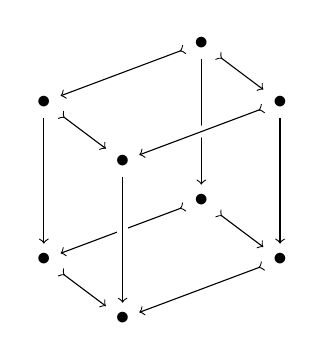
\begin{tikzpicture}
		\node (tb) at (2,2.75) {$\bullet$};
		\node (tl) at (0,2) {$\bullet$};
		\node (tr) at (3,2) {$\bullet$};
		\node (tf) at (1,1.25) {$\bullet$};
		\node (bb) at (2,0.75) {$\bullet$};
		\node (bl) at (0,0) {$\bullet$};
		\node (br) at (3,0) {$\bullet$};
		\node (bf) at (1,-.75) {$\bullet$};
		%
		\draw [>->] (tb) edge (tr);
		\draw [->] (tb) edge (bb);
		\draw [>->] (tb) edge (tl);
		\draw [->] (tr) edge (br);
		\draw [>->] (tl) edge (tf);
		\draw [->] (tl) edge (bl);
		\draw [>->] (bb) edge (br);
		\draw [>->] (bb) edge (bl);
		\draw [>->] (br) edge (bf);
		\draw [>->] (bl) edge (bf);
		%
		\draw [->] (tf) edge[white,line width=4pt] (bf);
		\draw [->] (tf) edge (bf);
		\draw [>->] (tr) edge[white,line width=4pt] (tf);
		\draw [>->] (tr) edge (tf);
		\end{tikzpicture}
	\]
	whose top and bottom faces consist of only monomorphisms. 
	If the top face is a pullback and the front faces are pushouts, 
	then the bottom face is a pullback if and only if the 
	back faces are pushouts.
\endlemma

A good portion of the theory for double pushout graph rewriting 
has been extended to adhesive categories. 
So, while our focus is on double pushout graph rewriting, 
there may be variations of the bicatgory $\cat{Rewrite}$ (introduced below) 
that are of interest to computer scientists.  For instance, 
the \emph{Schanuel topos} was used to model the $\pi$-calculus
	\cite{Fiore_OpModelsProcessCalulii} 
and adhesive categories allow us to extend rewriting to such settings.  
Our contribution is a bicategorical framework to house the rewriting as $2$-cells, 
though only for double pushout graph rewriting.

%%%%%%%%%%%
%	subsection:
%	rewriting
%	(bicat rewrite)
%%%%%%%%%%%

\subsection{$\cat{Rewrite}$}
\label{sec.Rewrite}

Here, we introduce the bicategory $\cat{Rewrite}$ as promised.  
To prepare, we begin by introducing a slight generalization 
of the double pushout graph rewriting concepts discussed above.  
An \emph{interface} $(I,O)$ is a pair of discrete graphs and a 
\emph{production with interface} $(I,O)$, or simply \emph{$(I,O)$-production}, 
is a cospan of spans
\[
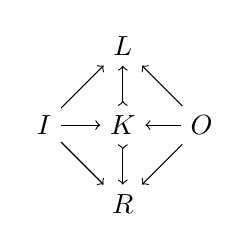
\begin{tikzpicture}
\node (I) at (-1,0) {$I$};
\node (O) at (1,0) {$O$};
\node (L) at (0,1) {$L$};
\node (K) at (0,0) {$K$};
\node (R) at (0,-1) {$R$};
%
\draw [->] (I) edge (L);
\draw [->] (I) edge (K);
\draw [->] (I) edge (R);
\draw [->] (O) edge (L);
\draw [->] (O) edge (K);
\draw [->] (O) edge (R);
\draw [>->] (K) edge (L);
\draw [>->] (K) edge (R);
\end{tikzpicture}
\]
Think of $I$ and $O$ as choosing inputs and outputs. 
Given a production with interface $(I,O)$, we say that a graph $G'$ is an 
\emph{$(I,O)$-derivation} of $G$ if there is a diagram
\[
	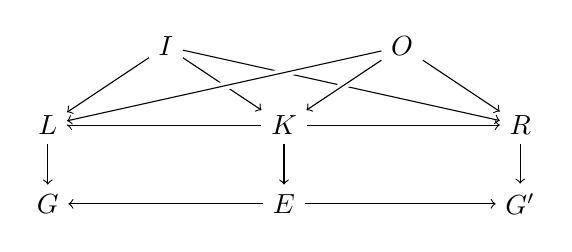
\begin{tikzpicture}
	\node (I) at (1.5,2) {$I$};
	\node (O) at (4.5,2) {$O$};
	\node (L) at (0,1) {$L$};
	\node (K) at (3,1) {$K$};
	\node (R) at (6,1) {$R$};
	\node (G) at (0,0) {$G$};
	\node (E) at (3,0) {$E$};
	\node (G') at (6,0) {$G'$};
	%
	\draw [->] (I) edge (L);
	\draw [->] (I) edge (K);
	\draw [->] (I) edge (R);
	\draw [->] (K) edge (L);
	\draw [->] (K) edge (E);
	\draw [->] (K) edge (R);
	\draw [->] (L) edge (G);
	\draw [->] (R) edge (G');
	\draw [->] (E) edge (G);
	\draw [->] (E) edge (G');
	%
	\draw [-] (O) edge[white,line width=3pt] (L);
	\draw [->] (O) edge (L);
	\draw [-] (O) edge[white,line width=3pt] (K);
	\draw [->] (O) edge (K);
	\draw [-] (O) edge[white,line width=3pt] (R);
	\draw [->] (O) edge (R);
	\end{tikzpicture}
\]
where the bottom squares are pushouts. We denote this as $G \rightsquigarrow G'$. 
An \emph{$(I,O)$-grammar} 
	$(\mathcal{G},\mathcal{P})$ 
consists of a collection of graphs $\mathcal{G}$ 
and another of $(I,O)$-productions $\mathcal{P}$. 
Again, an $(I,O)$-grammar generates a language 
consisting of all graphs $G$ such that there is a chain of $(I,O)$-derivations 
	$G_0 \rightsquigarrow 
		G_1 \rightsquigarrow \dotsm \rightsquigarrow 
		G_n=G$ 
from $\mathcal{P}$ such that $G_0 \in \mathcal{G}$. 
However, this time, we require such a chain to respect 
the inputs and outputs in the sense that 
	\begin{equation} \label{diag.DerivationChain}
		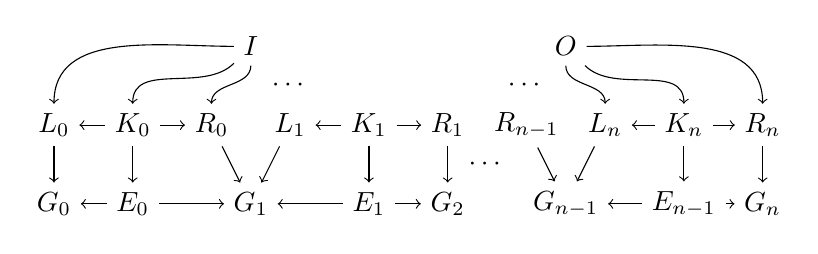
\begin{tikzpicture}
		\node (G0) at (0,-1) {$G_0$};
		\node (E0) at (1,-1) {$E_0$};
		\node (G1) at (2.5,-1) {$G_1$};
		\node (E1) at (4,-1) {$E_1$};
		\node (G2) at (5,-1) {$G_2$};
		\node (Gn-1) at (6.5,-1) {$G_{n-1}$};
		\node (En-1) at (8,-1) {$E_{n-1}$};
		\node (Gn) at (9,-1) {$G_n$};
		\node (L0) at (0,0) {$L_0$};
		\node (K0) at (1,0) {$K_0$};
		\node (R0) at (2,0) {$R_0$};
		\node (L1) at (3,0) {$L_1$};
		\node (K1) at (4,0) {$K_1$};
		\node (R1) at (5,0) {$R_1$};
		\node (Rn-1) at (6,0) {$R_{n-1}$};
		\node (Ln) at (7,0) {$L_n$};
		\node (Kn) at (8,0) {$K_n$};
		\node (Rn) at (9,0) {$R_n$};
		\node (I) at (2.5,1) {$I$};
		\node (O) at (6.5,1) {$O$};
		\node (dots) at (5.5,-0.5) {$\dotsm$};
		%
		\draw [->] (L0) edge (G0);
		\draw [->] (K0) edge (E0);
		\draw [->] (R0) edge (G1);
		\draw [->] (L1) edge (G1);
		\draw [->] (K1) edge (E1);
		\draw [->] (R1) edge (G2);
		\draw [->] (Rn-1) edge (Gn-1);
		\draw [->] (Ln) edge (Gn-1);
		\draw [->] (Kn) edge (En-1);
		\draw [->] (Rn) edge (Gn);
		\draw [->] (K0) edge (L0);
		\draw [->] (K0) edge (R0);
		\draw [->] (K1) edge (L1);
		\draw [->] (K1) edge (R1);
		\draw [->] (Kn) edge (Ln);
		\draw [->] (Kn) edge (Rn);
		\draw [->] (E0) edge (G0);
		\draw [->] (E0) edge (G1);
		\draw [->] (E1) edge (G1);
		\draw [->] (E1) edge (G2);
		\draw [->] (En-1) edge (Gn-1);
		\draw [->] (En-1) edge (Gn);
		%
		\draw [->] (I) edge[out=180,in=90] (L0);
		\draw [->] (I) edge[out=225,in=90] (K0);
		\draw [->] (I) edge[out=270,in=90] (R0);
		\draw [->] (O) edge [out=0,in=90] (Rn);
		\draw [->] (O) edge [out=-45,in=90] (Kn);
		\draw [->] (O) edge [out=-90,in=90] (Ln);
		%
		\node (Idots) at (3,0.5) {$\dotsm$};
		\node (Odots) at (6,0.5) {$\dotsm$};
		\end{tikzpicture}
	\end{equation}
Now we can put these productions with 
interfaces into our bicategorical framework.

Consider the full sub-bicategory of $\csC$ for 
	$\cat{C} \coloneqq \cat{Graph}$ 
with objects the finite, discrete graphs. 
Here, a $1$-cell is a cospan 
	$ G \from I \cospan O $ 
where $G$ is a graph and $I$, $O$ are discrete graphs.  
A $2$-cell between $1$-cells $G'$ and $G''$ is a span of cospans 
	$ G \from G' \span G'' $ 
which we think of as an $(I,O)$-derivation 
	$ G' \rightsquigarrow G'' $.  
We call this sub-bicategory $\cat{Rewrite}$ 
because the $2$-cells are exactly all the possible ways 
to rewrite one graph into another so that inputs and outputs are preserved. 
Given any $2$-cell 
	$ G \from G' \span G'' $ 
in $\cat{Rewrite}$, then the diagram 
\[
	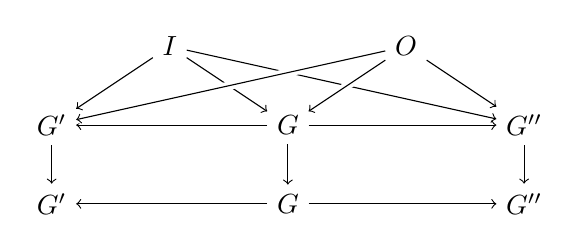
\begin{tikzpicture}
	\node (I) at (1.5,2) {$I$};
	\node (O) at (4.5,2) {$O$};
	\node (L) at (0,1) {$G'$};
	\node (K) at (3,1) {$G$};
	\node (R) at (6,1) {$G''$};
	\node (G) at (0,0) {$G'$};
	\node (E) at (3,0) {$G$};
	\node (G') at (6,0) {$G''$};
	%
	\draw [->] (I) edge (L);
	\draw [->] (I) edge (K);
	\draw [->] (I) edge (R);
	\draw [->] (K) edge (L);
	\draw [->] (K) edge (E);
	\draw [->] (K) edge (R);
	\draw [->] (L) edge (G);
	\draw [->] (R) edge (G');
	\draw [->] (E) edge (G);
	\draw [->] (E) edge (G');
	%
	\draw [-] (O) edge[white,line width=3pt] (L);
	\draw [->] (O) edge (L);
	\draw [-] (O) edge[white,line width=3pt] (K);
	\draw [->] (O) edge (K);
	\draw [-] (O) edge[white,line width=3pt] (R);
	\draw [->] (O) edge (R);
	\end{tikzpicture}
\]
gives an $(I,O)$-derivation 
	$ G' \rightsquigarrow_G G'' $. 
Conversely, any $(I,O)$-derivation 
	\eqref{diag.DerivationChain} 
can be made into composable $2$-cells 
	$ E_i \from G_i \span G_{ i + 1 }$ 
where the maps from $I$ and $O$ are the evident composites. 
Then, the vertical composition of the resulting $2$-cells 
gives us the desired span of cospans.

To better illustrate this, we provide a concrete 
example of the dictionary between $\cat{Rewrite}$ and 
double pushout graph rewriting.  
Suppose we were given an $(I,O)$-derivation with 
	$ I = \{ \ast \} = O $, 
induced from the following double pushout graph rewriting diagram
\[
	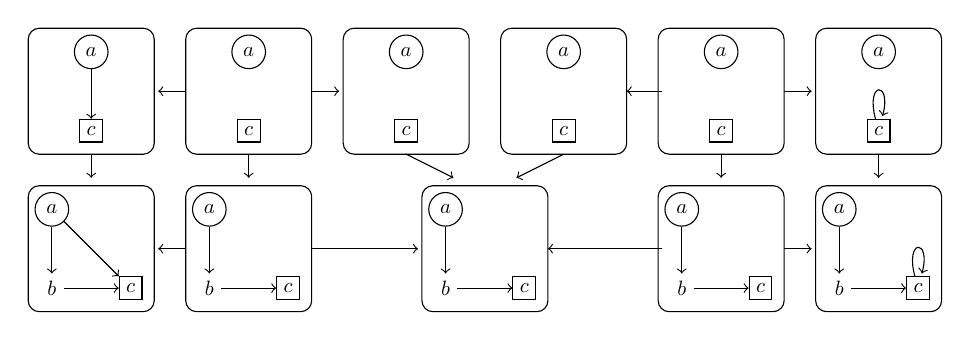
\begin{tikzpicture} 
	% TOP ROW BOXES
	\draw[rounded corners] (-0.3,1.7) rectangle (1.3,3.3);
	\draw[rounded corners] (1.7,1.7) rectangle (3.3,3.3);
	\draw[rounded corners] (3.7,1.7) rectangle (5.3,3.3);
	\draw[rounded corners] (5.7,1.7) rectangle (7.3,3.3);
	\draw[rounded corners] (7.7,1.7) rectangle (9.3,3.3);
	\draw[rounded corners] (9.7,1.7) rectangle (11.3,3.3);
	% BOTTOM ROW BOXES
	\draw[rounded corners] (-0.3,-0.3) rectangle (1.3,1.3);
	\draw[rounded corners] (1.7,-0.3) rectangle (3.3,1.3);
	\draw[rounded corners] (4.7,-0.3) rectangle (6.3,1.3);
	\draw[rounded corners] (7.7,-0.3) rectangle (9.3,1.3);
	\draw[rounded corners] (9.7,-0.3) rectangle (11.3,1.3);
	% TOP ROW GRAPHS
	\node[draw,circle,scale=0.75] (a1) at (0.5,3) {$a$};
	\node[draw,rectangle,scale=0.75] (c1) at (0.5,2) {$c$};
	\node[draw,circle,scale=0.75] (a2) at (2.5,3) {$a$};
	\node[draw,rectangle,scale=0.75] (c2) at (2.5,2) {$c$};
	\node[draw,circle,scale=0.75] (a3) at (4.5,3) {$a$};
	\node[draw,rectangle,scale=0.75] (c3) at (4.5,2) {$c$};
	\node[draw,circle,scale=0.75] (a4) at (6.5,3) {$a$};
	\node[draw,rectangle,scale=0.75] (c4) at (6.5,2) {$c$};
	\node[draw,circle,scale=0.75] (a5) at (8.5,3) {$a$};
	\node[draw,rectangle,scale=0.75] (c5) at (8.5,2) {$c$};
	\node[draw,circle,scale=0.75] (a6) at (10.5,3) {$a$};
	\node[draw,rectangle,scale=0.75] (c6) at (10.5,2) {$c$};
	% BOTTOM ROW GRAPHS
	\node[draw,circle,scale=0.75] (a7) at (0,1) {$a$};
	\node[scale=0.75] (b1) at (0,0) {$b$};
	\node[draw,rectangle,scale=0.75] (c7) at (1,0) {$c$};
	\node[draw,circle,scale=0.75] (a8) at (2,1) {$a$};
	\node[scale=0.75] (b2) at (2,0) {$b$};
	\node[draw,rectangle,scale=0.75] (c8) at (3,0) {$c$};
	\node[draw,circle,scale=0.75] (a9) at (5,1) {$a$};
	\node[scale=0.75] (b3) at (5,0) {$b$};
	\node[draw,rectangle,scale=0.75] (c9) at (6,0) {$c$};
	\node[draw,circle,scale=0.75] (a10) at (8,1) {$a$};
	\node[scale=0.75] (b4) at (8,0) {$b$};
	\node[draw,rectangle,scale=0.75] (c10) at (9,0) {$c$};
	\node[draw,circle,scale=0.75] (a11) at (10,1) {$a$};
	\node[scale=0.75] (b5) at (10,0) {$b$};
	\node[draw,rectangle,scale=0.75] (c11) at (11,0) {$c$};
	% GRAPH EDGES
	\draw [->] (a1) -- (c1);
	\draw (c6) edge [loop above] (c6);
	\draw [->] (a7) -- (b1);
	\draw [->] (b1) -- (c7);
	\draw [->] (a8) -- (b2);
	\draw [->] (b2) -- (c8);
	\draw [->] (a9) -- (b3);
	\draw [->] (b3) -- (c9);
	\draw [->] (a10) -- (b4);
	\draw [->] (b4) -- (c10);
	\draw [->] (a11) -- (b5);
	\draw [->] (a7) -- (c7);
	\draw [->] (b5) -- (c11);
	\draw (c11) edge [loop above] (c11);
	% BETWEEN BOX EDGES
	\draw [->] (1.7,2.5) -- (1.35,2.5);
	\draw [->] (3.3,2.5) -- (3.65,2.5);
	\draw [->] (7.75,2.5) -- (7.3,2.5);
	\draw [->] (9.3,2.5) -- (9.65,2.5);
	\draw [->] (1.7,0.5) -- (1.35,0.5);
	\draw [->] (3.3,0.5) -- (4.65,0.5);
	\draw [->] (7.75,0.5) -- (6.3,0.5);
	\draw [->] (9.3,0.5) -- (9.65,0.5);
	\draw [->] (0.5,1.7) -- (0.5,1.4);
	\draw [->] (2.5,1.7) -- (2.5,1.4);
	\draw [->] (4.5,1.7) -- (5.1,1.4);
	\draw [->] (6.5,1.7) -- (5.9,1.4);
	\draw [->] (8.5,1.7) -- (8.5,1.4);
	\draw [->] (10.5,1.7) -- (10.5,1.4);
	\end{tikzpicture}
\]
where the functions are described by the labeling, 
the inputs are circled, and the outputs are squared. 
In words, we have rewritten the graph on the lower left 
by removing an edge 
	$ a \to c $ 
and adding a loop 
	$ c \to c $. 
The pullback of the span
\[
	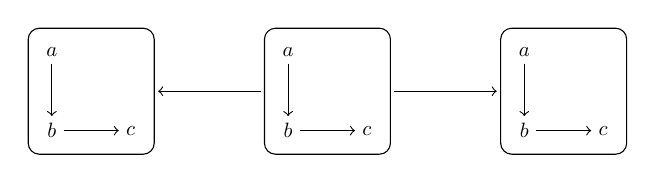
\begin{tikzpicture}
	\draw[rounded corners] (-0.3,-0.3) rectangle (1.3,1.3);
	\draw[rounded corners] (2.7,-0.3) rectangle (4.3,1.3);
	\draw[rounded corners] (5.7,-0.3) rectangle (7.3,1.3);
	%
	\node[scale=0.75] (a1) at (0,1) {$a$};
	\node[scale=0.75] (b1) at (0,0) {$b$};
	\node[scale=0.75] (c1) at (1,0) {$c$};
	\node[scale=0.75] (a2) at (3,1) {$a$};
	\node[scale=0.75] (b2) at (3,0) {$b$};
	\node[scale=0.75] (c2) at (4,0) {$c$};
	\node[scale=0.75] (a3) at (6,1) {$a$};
	\node[scale=0.75] (b3) at (6,0) {$b$};
	\node[scale=0.75] (c3) at (7,0) {$c$};
	%
	\draw [->] (a1) -- (b1);
	\draw [->] (b1) -- (c1);
	\draw [->] (a2) -- (b2);
	\draw [->] (b2) -- (c2);
	\draw [->] (a3) -- (b3);
	\draw [->] (b3) -- (c3);
	%
	\draw [->] (2.65,0.5) -- (1.35,0.5); 
	\draw [->] (4.35,0.5) -- (5.65,0.5);
	\end{tikzpicture}
\]
is the graph
\[
	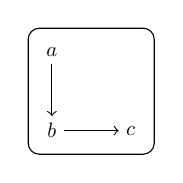
\begin{tikzpicture}
	\draw[rounded corners] (-0.3,-0.3) rectangle (1.3,1.3);
	%
	\node[scale=0.75] (a1) at (0,1) {$a$};
	\node[scale=0.75] (b1) at (0,0) {$b$};
	\node[scale=0.75] (c1) at (1,0) {$c$};
	%
	\draw [->] (a1) -- (b1);
	\draw [->] (b1) -- (c1);
	\end{tikzpicture}
\]
The corresponding $2$-cell is the diagram
\[
	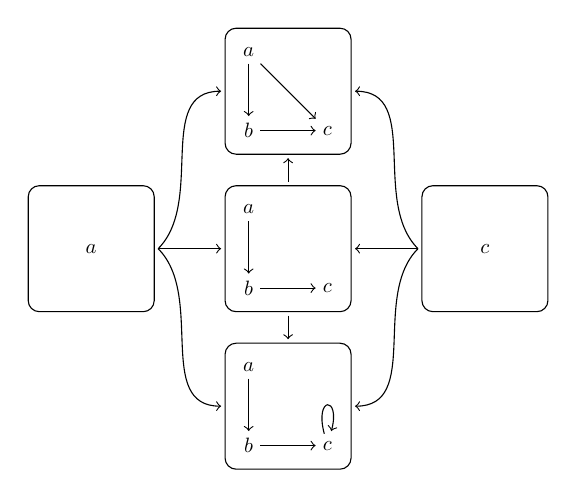
\begin{tikzpicture}
	\draw[rounded corners] (1.7,-0.3) rectangle (3.3,1.3);
	\draw[rounded corners] (1.7,1.7) rectangle (3.3,3.3);
	\draw[rounded corners] (1.7,3.7) rectangle (3.3,5.3);
	\draw[rounded corners] (-0.8,1.7) rectangle (0.8,3.3);
	\draw[rounded corners] (4.2,1.7) rectangle (5.8,3.3);
	%
	\node[scale=0.75] (ai) at (0,2.5) {$a$};
	\node[scale=0.75] (co) at (5,2.5) {$c$};
	\node[scale=0.75] (a1) at (2,5) {$a$};
	\node[scale=0.75] (b1) at (2,4) {$b$};
	\node[scale=0.75] (c1) at (3,4) {$c$};
	\node[scale=0.75] (a2) at (2,3) {$a$};
	\node[scale=0.75] (b2) at (2,2) {$b$};
	\node[scale=0.75] (c2) at (3,2) {$c$};
	\node[scale=0.75] (a3) at (2,1) {$a$};
	\node[scale=0.75] (b3) at (2,0) {$b$};
	\node[scale=0.75] (c3) at (3,0) {$c$};
	%
	\draw [->] (a1) edge (b1);
	\draw [->] (b1) edge (c1);
	\draw [->] (a2) edge (b2);
	\draw [->] (b2) edge (c2);
	\draw [->] (a3) edge (b3);
	\draw [->] (b3) edge (c3);
	\draw [->] (a1) edge (c1);
	\draw [->] (c3) edge [loop above] (c3);
	%
	\path [->] (0.85,2.5) edge (1.65,2.5);
	\path [->] (0.85,2.5) edge[out=45,in=180] (1.65,4.5);
	\path [->] (0.85,2.5) edge[out=-45,in=180] (1.65,0.5);
	\path [->] (4.15,2.5) edge (3.35,2.5);
	\path [->] (4.15,2.5) edge[out=135,in=0] (3.35,4.5);
	\path [->] (4.15,2.5) edge[out=225,in=0] (3.35,0.5);
	\draw [->] (2.5,3.35) -- (2.5,3.65);
	\draw [->] (2.5,1.65) -- (2.5,1.35);
	\end{tikzpicture}
\]
Here we witness the advantage that graph rewriting has 
over graph morphisms in the realm of expresivity. 
There is no way to replace the $2$-cell above 
with a map of graph cospans. 

There is nothing inherently special, 
from a mathematical point of view, 
about working with graphs and their morphisms.  
It is in applications where graphs gain importance.  
We can actually create categories analogous to 
$\cat{Rewrite}$ with any topos.  

%%%%%%%%%%%
%	section:
%	conclusion
%%%%%%%%%%%

\section{Conclusion and further work}

Our primary motivation for constructing this bicategory 
is as a way to study the gluing of graphs together in a way 
compatible with chosen input and output nodes. 
To this end, we defined a bicategory $\cat{Rewrite}$. 
This is a very large bicategory and in practice, 
one begins with a grammar and studies the resulting language. 
So, in an upcoming collaboration with Kenny Courser, 
we look at relating languages to sub-bicategories of $\cat{Rewrite}$ 
generated by a grammar. In this same paper, 
we study the structure of $\cat{MonSp(Csp(C))}$ alongside similar bicategories. 

%%%%%%%%%%%%
%
%	bibliography
%
%%%%%%%%%%%

\begin{references*}	
	\bibitem{Baader_TermRewritingAllThat}
	F.~Baader and T.~Nipkow.
	\newblock {\em Term {R}ewriting and {A}ll {T}hat}.
	\newblock Cambridge University Press, 1998.
	
	\bibitem{Baez_CompFrameMarkovProcess}
	J.~Baez, B.~Fong, and B.~Pollard.
	\newblock A {C}ompositional {F}ramework for {M}arkov {P}rocesses.
	\newblock {\em {J}. {M}ath. {P}hys.}, 57(3):033301, 2016.
	\newblock Available as
	\href{https://arxiv.org/abs/1508.06448}{arXiv:1508.06448}.
	
	\bibitem{Baez_CompFrameLinearNetworks}
	J.~C. Baez and B.~Fong.
	\newblock A {C}ompositional {F}ramework for {P}assive {L}inear {N}etworks.
	\newblock 2015.
	\newblock Available as
	\href{https://arxiv.org/abs/1504.05625}{arXiv:1504.05625}.
	
	\bibitem{Benabou_Bicats}
	J.~B{\'e}nabou.
	\newblock {\em Introduction to {B}icategories}, pages 1--77.
	\newblock Springer Berlin Heidelberg, Berlin, Heidelberg, 1967.
	
	\bibitem{Ehrig_GraphGramAlgAp}
	H.~Ehrig, M.~Pfender, and H.~J. Schneider.
	\newblock Graph-{G}rammars: An {A}lgebraic {A}pproach.
	\newblock In {\em Switching and Automata Theory, 1973. SWAT'08. IEEE Conference
		Record of 14th Annual Symposium on}, pages 167--180. IEEE, 1973.
	
	\bibitem{Fiore_OpModelsProcessCalulii}
	M.~Fiore and S.~Staton.
	\newblock Comparing {O}perational {M}odels of {N}ame-{P}assing {P}rocess
	{C}alculi.
	\newblock {\em Inform. Comput.}, 204 (4) : 524--560, 2006.
	\newblock Available at
	\href{http://www.cs.ox.ac.uk/people/samuel.staton/papers/cmcs04.pdf}{http://www.cs.ox.ac.uk/people/samuel.staton/papers/cmcs04.pdf}.
	
	\bibitem{GrandisPare_Intercats}
	M.~Grandis and R.~Par\'{e}.
	\newblock Intercategories.
	\newblock {\em Theor. Appl. Categ.}, 30(38):1215--1255, 2015.
	\newblock Available at
	\href{http://www.tac.mta.ca/tac/volumes/30/38/30-38.pdf}{http://www.tac.mta.ca/tac/volumes/30/38/30-38.pdf}.
	
	\bibitem{LackSoboc_AdhesiveCategories}
	S.~Lack and P.~Soboci{\'n}ski.
	\newblock Adhesive categories.
	\newblock In {\em Foundations of {S}oftware {S}cience and {C}omputation
		{S}tructures}, volume 2987 of {\em Lecture Notes in Comput. Sci.}, pages
	273--288. Springer, Berlin, 2004.
	\newblock Available at
	\href{ftp://ftp.daimi.au.dk/BRICS/RS/03/31/BRICS-RS-03-31.pdf}{ftp://ftp.daimi.au.dk/BRICS/RS/03/31/BRICS-RS-03-31.pdf}.
	
	\bibitem{LackSoboc_ToposesAdhesive}
	S.~Lack and P.~Soboci{\'n}ski.
	\newblock Toposes are {A}dhesive.
	\newblock In {\em Graph transformations}, volume 4178 of {\em Lecture Notes in
		Comput. Sci.}, pages 184--198. Springer, Berlin, 2006.
	\newblock Available at
	{\href{http://users.ecs.soton.ac.uk/ps/papers/toposesAdhesive.pdf}{http://users.ecs.soton.ac.uk/ps/papers/toposesAdhesive.pdf}}.
	
	\bibitem{MacLaneMoerdijk_SheavesGeomLogic}
	S.~Mac~Lane and I.~Moerdijk.
	\newblock {\em Sheaves in {G}eometry and {L}ogic}.
	\newblock Universitext. Springer-Verlag, New York, 1994.
	\newblock A first introduction to topos theory.
	
	\bibitem{Rebro_Span2}
	F.~Rebro.
	\newblock Building the {B}icategory {$\textbf{Span}_2 (C)$}.
	\newblock 2015.
	\newblock Available as
	\href{https://arxiv.org/abs/1501.00792}{arXiv:1501.00792}.
	
	\bibitem{RoseSabadinWalters_SepAlgNCospansGraphs}
	R.~Rosebrugh, N.~Sabadini, and R.~Walters.
	\newblock Generic {C}ommutative {S}eparable {A}lgebras and {C}ospans of
	{G}raphs.
	\newblock {\em Theor. Appl. Categ.}, 15(6):164--177, 2005.
	\newblock Available at
	\href{http://www.tac.mta.ca/tac/volumes/15/6/15-06.pdf}{http://www.tac.mta.ca/tac/volumes/15/6/15-06.pdf}.
	
	\bibitem{RoseSabadinWalters_CalcColimsComp}
	R.~Rosebrugh, N.~Sabadini, and R.~F. Walters.
	\newblock Calculating {C}olimits {C}ompositionally.
	\newblock In {\em Concurrency, Graphs and Models}, pages 581--592. Springer,
	2008.
	\newblock Available as \href{https://arxiv.org/abs/0712.2525}{arXiv:0712.2525}.
\end{references*}

%%%%%%%%%%%
%
% end document
%
%%%%%%%%%%%

\end{document}

